\chapter{Analýza}
\label{sec:an}

Před samotným návrhem a implementací nadřazeného systému je potřeba přesněji definovat požadavky na jeho vlastnosti a chování. Z~hlediska chování by systém měl poskytovat následující funkce:

\begin{itemize}
    \item Systém má být schopen komunikovat s~podřízenými systémy pomocí WiFi či Ethernetu (v~rámci místní sítě). Komunikace je založena na zasílání událostí zaznamenaných podřízenými systémy.
    \item Systém má uchovávat zaznamenané události, včetně data a času přijetí a podřízeného systému, který událost vytvořil.
    \item Systém má umožňovat správu pomocí webového rozhraní, které by mělo umožňovat následující funkce:
        \begin{itemize}
            \item Přidat (registrovat) či odebrat podřízený systém.
            \item Zobrazit stav registrovaných podřízených systémů.
            \item Zobrazit zaznamenané události.
            \item Měnit nastavení jednotlivých podřízených systémů.
            \item Měnit uživatelské nastavení.
        \end{itemize}
    \item Systém má být schopen informovat provozovatele při poplachu či poruše.
\end{itemize}

Dále jsou od nadřazeného systému požadovány tyto vlastnosti:

\begin{itemize}
    \item \textbf{Bezpečnost} -- jak komunikace s~podřízenými systémy, tak přístup do uživatelského rozhraní by měl probíhat přes zabezpečený komunikační kanál.
    \item \textbf{Spolehlivost} -- způsob komunikace i systém jako celek by měl být dostatečně spolehlivý.
    \item \textbf{Presistence} -- data v~systému by měla být uchovávána presistentním způsobem.
    \item \textbf{Nezávislost} -- systém by neměl být příliš závislý na externích službách a alespoň v~omezené míře fungovat i bez přístupu k~internetu.
\end{itemize}

Na základě těchto požadavků je tedy potřeba zvolit vhodné nástroje pro implementaci systému. To je v~první řadě komunikační protokol použitý pro komunikaci s~podřízenými systémy. Tento protokol by měl být dostatečně robustní, rozšířený a podporovat šifrování. Také by s~jeho pomocí mělo být možné bezpečně ověřit identitu podřízených systémů. Výběrem protokolu se zabývá sekce \ref{sec:an_protocol}.

Další důležitá volba je způsob uchování zachycených událostí a dalších údajů. Data je nutné uchovávát presistentně, nejlépe v~obecně používaném formátu, který umožní další zpracování i mimo nadřazený systém. Výběr úložiště je popsán v~sekci \ref{sec:an_data}.

Nadřazený systém má být také schopen upozornit uživatele v~případě hrozícího nebezpečí nebo výpadku podřízeného systému. To je možné provést mnoha způsoby, jejichž možnosti jsou shrnuty v~sekci \ref{sec:an_notify}.

Nakonec zbývá zvolit programovací jazyk a případně frameworky pro tvorbu aplikace. Vhodných jazyků je dnes velké množství, jde tedy spíše o~otázku osobní preference. Volbou programovacího jazyka se zabývá sekce \ref{sec:an_lang}.

Z~těchto požadavků vyplývá software potřebný k~implementaci nadřazeného systému, jehož dostupnost je hlavní požadavek při volbě hardwarové platformy v~sekci \ref{sec:an_plat}. 

\section{Struktura systému}
\label{sec:an_struct}

Struktura celého systému je naznačena na obrázku \ref{fig:basic_struct}. \textcolor{blue2}{Podřízené systémy} komunikují s~\textcolor{green}{nadřazeným} na základě událostí. Nadřazený systém tyto události zpracovává a upravuje podle nich stav garáží v~evidenci. 

Zaznamenané události jsou také uchovávány v~historii událostí, spolu s~dalšími metadaty jako čas přijetí nebo podřízeného systému, který událost vytvořil.

Komunikace mezi podřízeným a nadřazeným systémem je postavena na modelu \textit{client/server}. Nadřazený systém provozuje server zvoleného protokolu (viz sekci \ref{sec:an_protocol}), ke kterému se podřízené systémy připojují. Komunikaci tedy vždy iniciuje podřízený systém. S~možností zasílání nevyžádaných zpráv podřízeným systémům v~této práci nepočítám, mohl by to však být námět pro další rozšíření.

Další, kdo přistupuje do systému, je \textcolor{magenta}{uživatel}. Přes webové rozhraní může sledovat stav garáží a historii událostí. Také zde může spravovat klíče, které slouží pro přístup ke komunikačnímu API systému. Přístup do webového rozhraní je zabezpečen heslem.

\begin{figure}[h!]
    \centering
    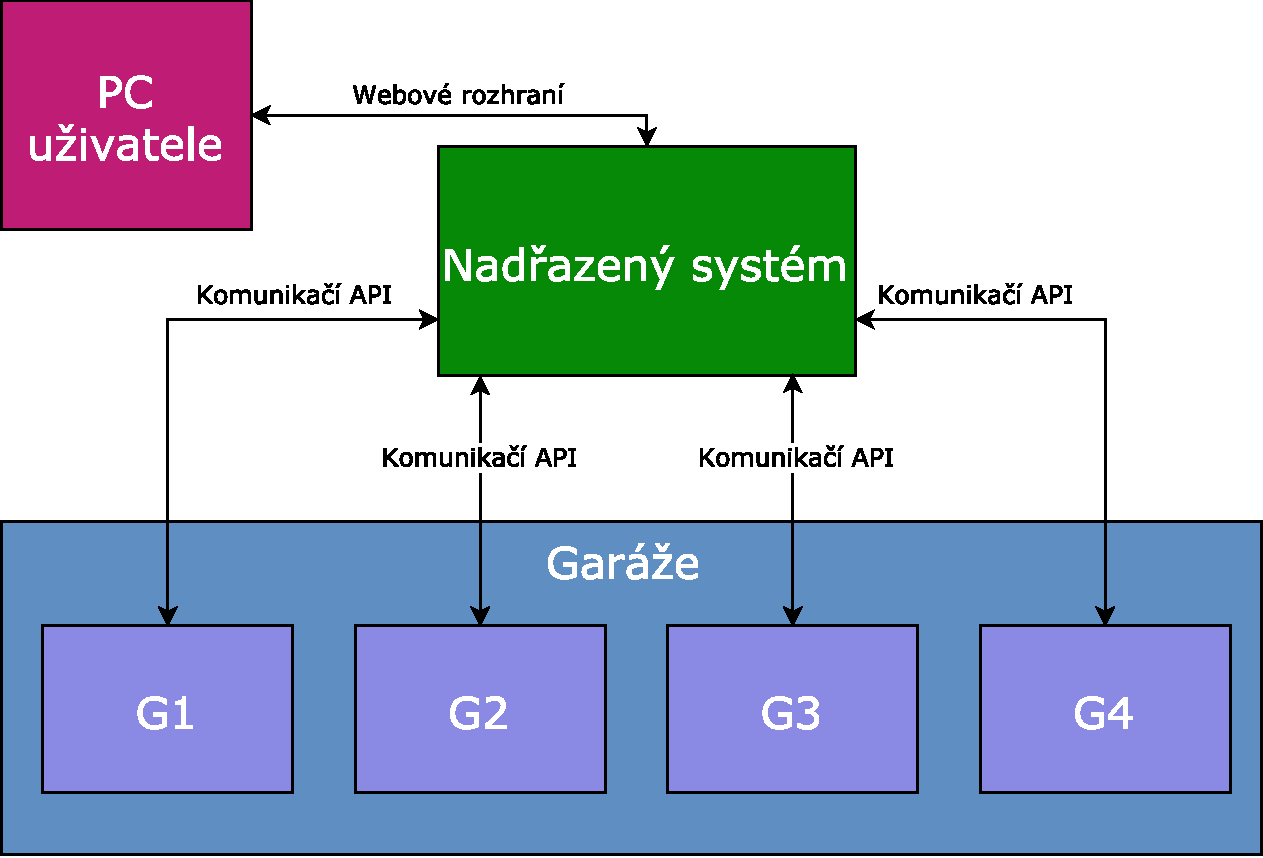
\includegraphics[width=\textwidth]{images/basic_struct.pdf}
    \caption[Základní struktura systému]{Základní struktura systému. Podřízené systémy využívají komunikační API k~zasílání událostí. Nadřazený systém tyto události zaznamenává a upravuje podle nich stav garáží. Uživatel nadřazený systém ovládá pomocí webového rozhraní. }
    \label{fig:basic_struct}
\end{figure}

\subsection{Podřízený systém}

Podřízený systém je zařízení umístěné v~každé garáži, které sleduje stav okolí pomocí těchto senzorových vstupů:

\begin{itemize}
    \item detekce kouře,
    \item detekce pohybu,
    \item stav dveří.
\end{itemize}

Základní požadavek na podřízený systém je schopnost komunikace přes Ethernet či WiFi pomocí protokolu zvoleného v~sekci \ref{sec:an_protocol}. Jinak může být hardware prakticky libovolný.

Návrh a implementace podřízeného systému není součástí této práce. Jeho vývojem se zabývá Miroslav Váňa ve své bakalářské práci na Katedře číslicového návrhu Fakulty informačních technologií ČVUT.

\subsection{Událost}

Událost slouží jako základní komunikační jednotka mezi nadřazeným a podřízeným systémem. V~případě překročení mezních hodnot senzorů se jednotlivé podřízené systémy okamžitě hlásí nadřazenému systému. Kromě toho také v~pravidelných intervalech odesílají kontrolní hlášení. 

Vyhodnocení události je provedeno nadřazeným systémem. Podřízený systém tedy hlásí každou událost (například otevření dveří), aniž by nějak zkoumal její závažnost.

\section{Výběr komunikačního protokolu}
\label{sec:an_protocol}

Nejdřív je nutné určit způsob komunikace, který bude systém používat. Díky tomu se budu při vybíraní platformy moci ujistit, že jsou dostupné vhodné knihovny a další software. 

Nadřazený systém bude se svými klienty (monitorovací zařízení v~jednotlivých garážích) komunikovat přes WiFi nebo Ethernet. Základem komunikace bude TCP/IP protokol, je však potřeba zvolit vhodný protokol z~aplikační vrstvy OSI modelu, který na něm bude stavět.

\subsection{Vlastní protokol}

Jedna z~možností je implementovat vlastní protokol pomocí TCP/IP socketů. Toto řešení se mi však nezdá příliš vhodné, neboť nepřináší žádné významné výhody, naopak se s~ním pojí řada komplikací.

Pro vlastní protokol by bylo nutné vytvořit robustní server, který zvládá obsluhu více klientů najednou. Dále by vzhledem k~citlivosti přenášených dat bylo nutné implementovat nějakou formu šifrování. Tyto velmi obsáhlé problémy přitom řeší většina dnešních protokolů.

Další nevýhodou je nutnost implementace klientské části protokolu při vytváření nových zařízení spravovaných nadřazeným systémem. To do jisté míry omezuje jeho rozšiřitelnost.

\subsection{Protokol HTTPS}
\label{sec:an_https}

Další možnost je využít ke komunikaci protokol HTTPS. V~tomto případě by klienti komunikovali se sytémem pomocí HTTP metod jako například \verb|get| nebo \verb|post|.

Jelikož součástí požadavků na systém je i webové uživatelské rozhraní, bude v~každém případě nutné použít webový server pro jeho provoz. Ten by pak bylo možné využít i k~poskytnutí API pro komunikaci systému s~podřízenými systémy.

Vhodný webový server (jako například Apache \cite{apache_faq}) zajistí vícevláknovou obsluhu všech klientů. Protokol se také postará o~šifrování přenášených dat, je však nutné získat certifikát k~ověření pravosti serveru (viz sekci \ref{sec:an_certs}).

Certifikát bude potřeba zajistit i v~případě, že komunikace s~klienty nebude postavena na tomto protokolu. Je totiž nutné také zabezpečit webové rozhraní, například kvůli ověření totožnosti uživatele při přihlašování. Nutnost pořízení certifikátu tedy nepředstavuje nevýhodu oproti jiným protokolům. 

API realizované pomocí tohoto protokolu je poměrně snadno rozšiřitelné. Pro nově implementovanou operaci stačí definovat URL a případně formát přenášených dat.

Výhodou je také snadná implementace na straně klienta, tedy podřízeného systému. Knihovny realizující klientskou část protokolu jsou dostupné na většině populárních platforem jako například Arduino (s~Ethernet \textit{shieldem}, oficiální knihovna EthernetClient \cite{ard_web}) nebo ESP8266 (knihovna esp8266wifi \cite{esp_web}).

\subsubsection{Certifikáty pro provoz HTTPS}
\label{sec:an_certs}

Pro provoz HTTPS serveru lze použít například certifikáty certifikační autority Let's Encrypt, které jsou poskytovány  zdarma \cite{lets_encrypt_faq}. Kromě toho dodává Let's Encrypt také automatizačního klienta Certbot \cite{certbot} pro snadné nasazení a aktualizaci jejich certifikátů. Bohužel certifikáty jsou vydávány pouze na doménu \cite{lets_encrypt_faq}, což komplikuje použití v~místní síti.

Jiná možnost je použití \textit{self-signed} certifikátu \cite{cert_wallen}. Tento certifikát není podepsaný žádnou certifikační autoritou, ale pouze vlastníkem certifikátu. Může tedy sloužit k~šifrování komunikace (poskytuje veřejný klíč), ale je zranitelný vůči \textit{man-in-the-middle} útoku \cite{cert_wallen}.

\textit{Self-signed} certifiát však lze použít k~šifrování komunikace na uzavřené lokální síti, za předpokladu, že je server s~certifikátem (přesněji s~jeho soukromým klíčem) dostatečně zabezpečen \cite{cert_wallen}. 

Nevýhodou tohoto řešení je nedůvěra webových klientů (certifikát není podepsán certifikační autoritou a nelze tedy ověřit jeho pravost), což by ovlivnilo přístup k~uživatelskému rozhraní a API systému. V~případě webového rozhraní by prohlížeč zobrazil varování o~neznámém certifikátu. To by však mohl uživatel ignorovat. 

Podřízené systémy by při zasílání požadavků museli přeskočit krok ověření totožnosti serveru. Jak toho dosáhnout například v~knihovně Requests (umožňující vytváření HTTP požadavků \cite{requests}) pro jazyk Python \cite{python_tutorial} je naznačeno v~ukázce \ref{lst:req_selfsigned}. 

Tento jazyk a knihovna byly zvoleny z~důvodů kompaktnosti ukázkového kódu, v~jiných jazicích lze tuto verifikaci obejít obdobným způsobem.

\begin{listing}[htbp]
\caption{\label{lst:req_selfsigned} Vytvoření HTTPS požadavku v~knihovně Requests, bez ověření totožnosti serveru.}
\begin{minted}[bgcolor=codebg]{python}
>>> import requests
>>> r = requests.get('https://test.local/hello', verify=False)
>>> r.status_code
200
\end{minted}
\end{listing}

\subsubsection{Autentizace klientů na HTTPS}

Přístup k~API nadřazeného systému by měl být povolen pouze ověřeným klientům. Díky tomu bude možné zabránit například zasílání nepravdivých informací z~neznámých zdrojů.

Jednoduchou autentizaci přes HTTPS lze realizovat například pomocí generování API klíčů. Pro každý podřízený systém bude vygenerován klíč, kterým se při zasílání požadavku systém prokáže. Seznam platných klíčů by byl udržován v~databázi nadřazeného systému. Klíče by uživatel mohl přidávat nebo odebírat (například v~případě odcizení podřízeného systému) pomocí webového rozhraní.

Tyto klíče by také bylo nutné nahrát a uchovávat na podřízených systémech. Detaily tohoto procesu by záležely na platformě těchto systémů. Například u~Arduina by šlo klíč nahrát z~uživatelova počítače pomocí sériové linky (s~USB převodníkem) a udržovat ho v~paměti EEPROM, která je uchována i po odpojení napájení \cite{ard_eeprom}.

Také by bylo možné implementovat v~nadřazeném systému \uv{registrační mód}, který by bylo možné dočasně povolit ve webovém rozhraní. V~tomto módu by systém po přijetí speciálního API požadavku vygeneroval nový klíč. Ten by si uložil do své databáze platných klíčů, a také ho v~odpovědi zaslal žádajícímu zařízení. Pokud by mód povolen nebyl, odpovědel by systém chybovým kódem, například 403 -- \textit{Forbidden}. Zaslání požadavku z~podřízeného systému by mohlo být provedeno stisknutím tlačítka.

Tento přístup by byl pravděpodobně uživatelsky příjemnější, přináší však potencionální bezpečnostní rizika. Například pokud by uživatel zapomněl mód vypnout, systém by byl otevřený k~registraci nežádoucích zařízení. Takový problém by se však dal řešit například automatickou deaktivací módu po uplynutí časového limitu.

Útočník snažící se získat klíč k~API by také mohl periodicky zkoušet registrační požadavek a čekat na aktivaci módu. Obrana proti tomuto útoku by byla složitější, šlo by například filtrovat IP adresy s~příliš častými požadavky.

Obecně vycházím z~toho, že i v~případě registrace nežádoucího zařízení nemůže toto zařízení krátkodobě způsobit výraznější škody -- do databáze nadřazeného systému může pouze zasílat nová data, která jsou navíc vázana k~jeho identitě (API klíči). Nemůže tedy získávat data od jiných podřízených systému či měnit jejich záznamy. Neautorizované zařízení se také objeví v~seznamu registrovaných API klíčů, kde může být snadno odhaleno. 

\subsection{Protokol MQTT}
\label{sec:an_mqtt}

MQTT je komunikační protokol založený na modelu \textit{publisher/subscriber}, určený pro použití v~prostředí s~omezenými zdroji (malý výkon procesoru, omezená paměť atd.) \cite{mqtt_valerie}.

Komunikace mezi jednotlivými klienty v~systému je zprostředkována pomocí centrály, nazývané \textit{broker}. Ta spravuje adresy -- \textit{topics} -- na kterých mohou klienti publikovat či odebírat zprávy.

\begin{figure}[h!]
    \centering
    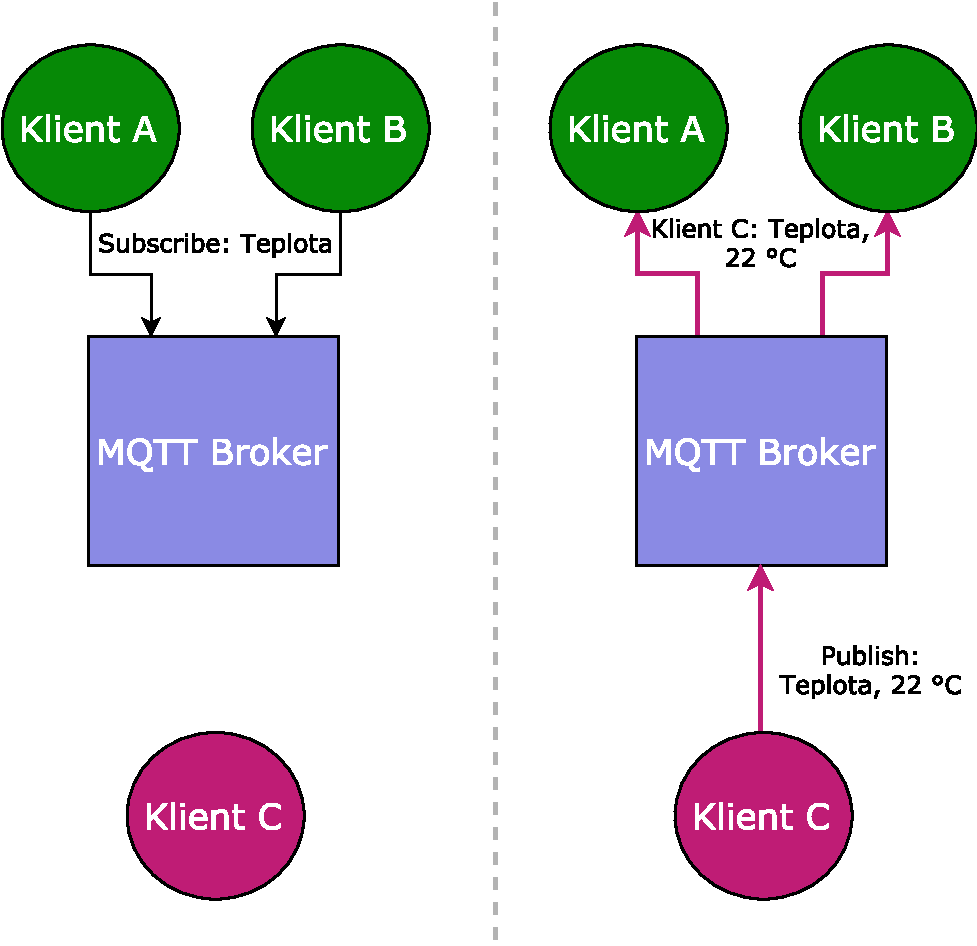
\includegraphics[width=\textwidth]{images/basic_mqtt.pdf}
    \caption[Příklad struktury protokolu MQTT]{Příklad struktury protokolu MQTT \cite{mqtt_eclipse}. Klienti A~a B jsou \textit{subscribery} \textit{topicu} \uv{Teplota}. Když klient C na tuto adresu publikuje novou zprávu, \textit{broker} se postará o~její doručení všem \textit{subscriberům}.}
    \label{fig:basic_mqtt}
\end{figure}

Na obrázku \ref{fig:basic_mqtt} tedy klienti \textcolor{green}{A} a \textcolor{green}{B} začnou odebírat \textit{topic} \uv{Teplota}. Když pak klient \textcolor{magenta}{C} pak publikuje zprávu na tuto adresu, \textcolor{blue2}{\textit{broker}} se postará o~doručení všem odebírajícím klientům.

Adresy je možné hierarchicky strukturovat následujícím způsobem \cite{mqtt_eclipse}: 

\begin{itemize}

\item Lze tvořit skupiny, například:
    \begin{itemize}
        \item \verb|/senzory/obyvak/teplota|.
        \item \verb|/senzory/kuchyne/vlhkost|.
    \end{itemize}
\item Zprávy je nutné publikovat na jednoznačnou adresu.
\item Při odebírání je možné použít modifikátory pro specifikování skupiny adres:
    \begin{itemize}
        \item Modifikátor \verb|+| -- odpovídá libovolnému jednomu stupni hierarchie. Například pro odebírání všech senzorů vlhkosti lze použít adresu \verb|/senzory/+/vlhkost|.
        \item Modifikátor \verb|#| -- odpovídá libovolnému počtu libovolných stupňů. Adresa \verb|/senzory/#| tedy slouží k~odebírání všech dat.
    \end{itemize}
\end{itemize}

V~případě této práce by tedy jak nadřazený systém, tak podřízené systémy byly klienty \textit{brokeru}. Podřízené systémy by publikovaly naměřená data, která by nadřazený systém odebíral. Tím by vznikla obdoba \textit{client/server} modelu, zmíněného v~sekci \ref{sec:an_struct}. 

Samotný \textit{broker} by pak mohl běžet souběžně s~nadřazeným systémem na zvolené platformě (například open-source \textit{broker} Mosquitto je dostupný na řadě platforem, včetně Raspberry Pi \cite{mqtt_mosquitto_wiki}).

Protokol podporuje tři možnosti QoS \cite{mqtt_valerie}:

\begin{itemize}
    \item Nejvýše jedno doručení -- tento mód pouze odešle zprávu, není zahrnut žádný opakovací mechanismus pro případ nedoručení.
    \item Alespoň jedno doručení -- v~tomto módu je zaručeno doručení zprávy, ta však může být doručena vícekrát.
    \item Přesně jedno doručení -- zde je ošetřeno i duplicitní doručování zpráv.
\end{itemize}

Použití sofistikovanějších metod doručení má vliv na výkon, a proto se v~některých případech vyplatí zvolit nižší úroveň QoS (například při posílání idempotentních zpráv). Pro tuto práci bych však pravděpodobně zvolil záruku přesně jednoho doručení.

\subsubsection{Šifrování a autentizace na MQTT}

V~této části se budu zabývat prostředky pro šifrování komunikace, které jsou dostupné v~\textit{brokeru} Mosquitto.

První možnost je pro zabezpečení komunikace využít certifikáty, podobně jako u~HTTPS. Zde by se pravděpodobně také využil \textit{self-signed} certifikát (blíže popsaný v~sekci \ref{sec:an_certs}). Mosquitto navíc také vyžaduje kořenový certifikát certifikační autority \cite{mqtt_mosquitto_tsl}. Při použití \textit{self-signed} ceritifikátů by bylo nutné tuto autoritu vytvořit a používané certifikáty u~ní podepsat (pro bližší informace viz \cite{ca_nguyen}). Kořenový certifikát by také bylo nutné distribuovat klientům.

Kromě certifikátů lze pro šifrování použít i PSK. V~tom případě \textit{broker} a jeho klienti používají pro zašifrování komunikace společný klíč (známý jak klientovi, tak \textit{brokeru}). Různí klienti přitom mohou mít různé klíče. \cite{mqtt_mosquitto_conf}

Bohužel podpora PSK v~MQTT klientech není příliš rozšířená. PSK je možné použít v~knihovně libmosquitto, určené pro C/C++ (s~vazbami pro Python). U~této knihovny se mi však podařilo najít pouze manuálovou stránku (viz \cite{libmosquitto_man}), bez informací o~jejím dalším vývoji či udržování. Modul poskytující vazby do Pythonu byl nicméně předán projektu Paho \cite{mosquitto_python}.

Paho poskytuje implementace MQTT klientů pro mnoho platforem (včetně například Arduina \cite{paho_embedded}). Dokumentace klientů pro C++ a Python však možnost šifrování pomocí PSK vůbec nezmiňuje \cite{paho_cpp_doc, paho_pyt_doc}.

Tyto možnosti lze použít i k~autentizaci klientů \textit{brokeru}. Při použití certifikátů lze v~konfiguračním souboru Mosquitta zvolit \verb|require_certificate| \cite{mqtt_mosquitto_conf}. Poté bude od klienta vyžadován certifikát prokazující jeho totožnost. Při použití PSK lze k~autentizaci využít sdílený klíč (\textit{broker} odmítne klienty s~neplatnými klíči) \cite{mqtt_mosquitto_conf}. Kromě toho je možno použít také autentizaci pomocí uživatelského jména a hesla, která je součástí MQTT protokolu, případně klienty neověřovat vůbec (a pouze šifrovat komunikaci) \cite{mqtt_mosquitto_conf}.

\subsection{Závěr výběru protokolu}

V~sekcích \ref{sec:an_https} a \ref{sec:an_mqtt} jsem se blíže podíval na dva poměrně rozšířené protokoly aplikační vrstvy, které by bylo možné použít pro tvorbu nadřazeného systému.

Pokud by mezi požadavky na systém bylo zahrnuto zasílání nevyžádaných zpráv podřízeným systému (jak je zmíněno v~sekci \ref{sec:an_struct}), zvolil bych pravděpodobně protokol MQTT. V~tom je tato funkcionalita velmi snadno implementovatelná -- stačí aby podřízené systémy odebíraly \textit{topic}, na kterém by nadřazený systém publikoval zprávy.

Jelikož se však v~této práci zabývám systémem, který zprávy pouze přijímá a zaznamenává, rozhodl jsem se pro HTTPS. Nasazení tohoto protokolu je o~něco snazší (není potřeba na zařízení instalovat \textit{broker} a zařizovat certifikační autoritu -- stačí \textit{self-signed} certifikát) a s~jeho použitím mám více zkušeností. Také se částečně uvolní požadavky na volbu platformy (webový server bude potřeba v~každém případě, při volbě HTTPS jako komunikačního protokolu mezi systémy tedy nebude nutný žádný další software). 

Každopádně bude mým cílem navrhnout výslednou aplikaci tak, aby rozhraní pro podřízené systémy realizované pomocí HTTPS bylo možné snadno nahradit MQTT rozhraním.

K~zabezpečení komunikace (včetně webového rozhraní) použiju \textit{self-signed} certifikát. Hlavní důvod je požadavek na použití v~místní síti, bez zaručeného přístupu k~internetu. Toto rozhodnutí nemá vliv na návrh a implementaci systému, pouze na jeho nasazení -- konkrétně konfiguraci webového serveru.

Pokud by provozovatel plánoval mít systém přístupný z~internetu (přes registrovanou doménu), musí v~každém případě k~zabezpečení použít certifikát podepsaný důvěryhodnou certifikační autoritou. Pak stačí pouze v~konfiguračním souboru webového serveru nahradit \textit{self-signed} certifikát podepsaným certifikátem. Není tedy nutné provádět změny v~kódu aplikace.

\section{Ukládání dat}
\label{sec:an_data}

Zaznamenané události bude potřeba presistentně uchovávat. Zde by šly využít jednoduché textové logy, vhodnější však bude zvolit nějaký databázový systém -- například kvůli širším možnostem zpracování naměřených údajů.

Z~dostupných možností mě zaujal SQLite, což není klasický databázový stroj s~modelem \textit{client/server}, ale místo toho tvoří součást programu, který databázi používá. Přístup k~datům je realizován pomocí přímého čtení/zápisu do databázového souboru na disku.  Díky tomu má malé nároky na diskový prostor a operační paměť. \cite{sqlite_about}

Jelikož bude nadřazený systém pravděpodobně provozován na hardwaru s~omezenými zdroji, představují tyto vlastnosti nezanedbatelnou výhodu. Použití SQLite také zjednouší nasazení aplikace, neboť nebude nutné vytvářet a konfigurovat databázový server.

\subsection{Velikost databáze}

Vzhledem k~požadavku na spolehlivost systému je vhodné odhadnout předpokládaný růst velikosti databázového souboru. Přiliš velká databáze by mohla vyčerpat pamět zařízení, a způsobit tak jeho pád. Také by mohla negativně ovlivnit dobu odezvy nadřazeného systému.

Pokud by se ukázalo, že při dlouhodobém provozu začíná být databáze neúnosně velká, bylo by nutné omezit množství uchovávaných dat, například pomocí front zaznamenaných událostí.

Při odhadu jsem vycházel z~předpokladu, že největší objem dat v~databázi budou představovat zaznamenaná kontrolní hlášení podřízených systému. Pokud se budou podřízené systémy hlásit každou hodinu, představuje 24 záznamů denně na každou garáž, což by mělo být řádově více než u~jiných událostí. Například u~pravděpodobně druhé nejčastější události, tedy otevření/zavření dveří, předpokládám nejvýše jednotky denně.

Událost kontrolního hlášení by měla obsahovat tyto údaje:

\begin{itemize}
    \item Identifikátor události v~databázi.
    \item Identifikátor garáže, ke které událost patří.
    \item Datum a čas zaznamenání události.
    \item Datum a čas dalšího plánovaného hlášení.
\end{itemize}

Jako identifikátory pravděpodobně budou stačit 32bitová celá čísla. Datum je možné v~SQLite ukládat buď jako textový retězec ve formátu \texttt{YYYY-MM-DD HH:MM:SS.SSS}, 64bitové reálné číslo, či 32bitové cele číslo -- \textit{Unix Time} \cite{sqlite_datetypes}. Z~toho vyplývá, že jedno kontrolní hlášení bude mít velikost alespoň $4 * 32 = 128$ bitů.

Pokud nadřazený systém monitoruje 30 garáží, kde každá odesílá kontrolní hlášení každou hodinu, jsou každý den vytvořeny záznamy o~velikosti $30 * 24 * 96 = 98304$ bitů, tedy asi 98 Kb. Dá se tedy předpokládat, že velikost databázového souboru neporoste nijak dramaticky.

Tento výpočet představuje pouze odhad předpokládané velikosti. Skutečná velikost bude záležet na zvolené implementaci, neměla by se však výrazně lišit od tohoto odhadu.

%v implementaci este popsat zmeny voproti tomuhle vodhadu, mozna taky doplnit aktualizovanej vypocet

\section{Zasílání notifikací}
\label{sec:an_notify}

Nadřazený systém má být schopen zasílat uživatelům notifikace o~stavu jednotlivých garáží. Notifikace mohou informovat o~důležité události (například detekce kouře) nebo o~výpadku podřízeného systému (v~případě promeškání plánovaného kontrolního hlášení).

Tyto notifikace by měl obdržet jednak správce garáží (provozovatel nadřazeného systému), jednak jednotlivý nájemci, kterým budou zasílány notifikace týkající se jejich garáže.

\subsection{E-mailové notifikace}

První možnost je zasílat notifikace pomocí e-mailu. K~tomu je zapotřebí vytvořit účet, který by mohl nadřazený systém použít k~odesílání.

Zde se nabízí možnost provozovat e-mailový server s~účtem přímo na zařízení, na kterém poběží nadřazený systém. Provoz takového serveru je však velmi náročný, a to nejen kvůli složité počáteční konfiguraci, ale také z~hlediska dlouhodobé údržby \cite{email_dont}. Tento přístup by tak kladl neúměrné nároky na uživatele systému.

Alternativa je použít nějakého poskytovatele e-mailových služeb, jako například Gmail od společnosti Google. Zde by si uživatel vytvořil účet určený k~odesílání notifikací, a poté autorizoval nadřazený systém k~odesílání zpráv z~tohoto účtu. 

Tímto je částečně porušen požadavek na nezávislost (viz sekci \ref{sec:an}). Při zasílání notifikací je však nutný přístup k~internetu i v~případě použití vlastního e-mailového serveru a nezávislost na externí službě nevyváží komplikace spojené s~jeho provozem.

%napsat problem se smtp prihlasenim (login a heslo musi bejt nekde v plaintextu). alternativa oauth u google nebo naky api

%napsat vo srani se s autentikaci u google

%napsat vo srani se jinejma mail sluzbama -- mailgun, sendgrid

%na email serem zkusime sms 

\subsection{SMS notifikace}

%cool moznost -- vlastni gsm modul, vyhody -- hlavne nezavislost (de i bez netu), kompatibilni s hafem hw (staci seriova linka, komunikace pomoci at commandu), knihovny/programy (gammu) pro snadny vovladani. nevyhody -- spatna kontrola (kredit -- jako cist kredit asi de nak pres ty ussd zpravy ale celej ten interface by se musel naprogramovat a v tim twilliu je proste uz hotovej, varovani vo zruseni simky atd), nutnost mit ten modul (nefungovalo by pri nasazeni v cloudu), muze bejt relativne drahej (jak modul tak samotny sms), nutnost sehnat simku, pri zruseni simky problem zjistit ze se to stalo, gammu nema knihovnu pro python3

%dalsi moznost twilio -- sluzba na posilani sms. vyhody -- relativne jednoduchy pouziti, snadna kontrola nad utratou, naky fancy pokrocily moznosti (custom cisla atd), levny (smsky, neni potreba gsm modul), comfy knihovna pro python3, snadna implementace, je mozny to pouzit i v tim cloudu. nevyhody -- potrebuje internet, nutna registrace (+ vyplneni kreditni karty, ale srovnat se shanenim sim karty), (trosicku slozitejsi na pouziti pro uzivatele -- musi vyplnit tri veci v tim web rozhrani).

\section{Programovací jazyk pro tvorbu systému}
\label{sec:an_lang}

Pro tvorbu systému jsem se rozhodl použít programovací jazyk Python \cite{python_tutorial}. S~tímto jazykem mám nejvíce zkušeností co se týče implementace webových aplikací. Je také dostatečně rozšířený, takže výsledný systém bude možné nasadit na poměrně širokém spektru platforem bez nutnosti složitějšího portování.

K~vytvoření webového rozhraní i API pro podřízené systémy jsem zvolil framework Flask \cite{flask_about}. Hlavní důvod jsou opět předchozí zkušenosti s~tímto frameworkem. Flask také dává více volnosti při návrhu aplikace než například také velmi rozšířený framework Django \cite{django_about}.

\section{Výběr platformy}
\label{sec:an_plat}

Pro realizaci systému je nutné zvolit vhodnou platformu. Jelikož je cílem práce vytvořit fyzické zařízení, rozhodl jsem se jako základ použít některý z~jednodeskových počítačů, které jsou v~dnešní době na trhu. Tyto počítače bývají cenově velmi dostupné a zároveň poskytují dostatečný výkon a podporu pro provoz systému.

Při výběru počítače byla nejdůležitejším kritériem podpora softwaru potřebného k~implementaci monitorovacího systému. Na základě předchozí analýzy je tedy vyžadován následující software:

\begin{itemize}
    \item Webový server Apache2.
    \item Databázový systém SQLite.
    \item Programovací jazyk Python 3.
    \begin{itemize}
        \item Webový framework Flask.
    \end{itemize}
\end{itemize}

Pro provoz tohoto softwaru bude potřeba plnohodnotný operační systém, což vylučuje platformy využívající jednoduché mikrokontroléry, jako například Arduino Uno. Kromě toho je nutné připojení k~síti pomocí Ethernetu nebo WiFi. 

V~dalších sekcích jsem se blíže podíval na jednodeskové počítače Raspberry Pi (sekce \ref{sec:an_rpi}) a Zybo Zynq-7000 (sekce \ref{sec:an_zyb}) a zvážil jejich výhody a nevýhody pro implementaci systému.

\subsection{Raspberry Pi}
\label{sec:an_rpi}

\begin{figure}[h!]
    \centering
    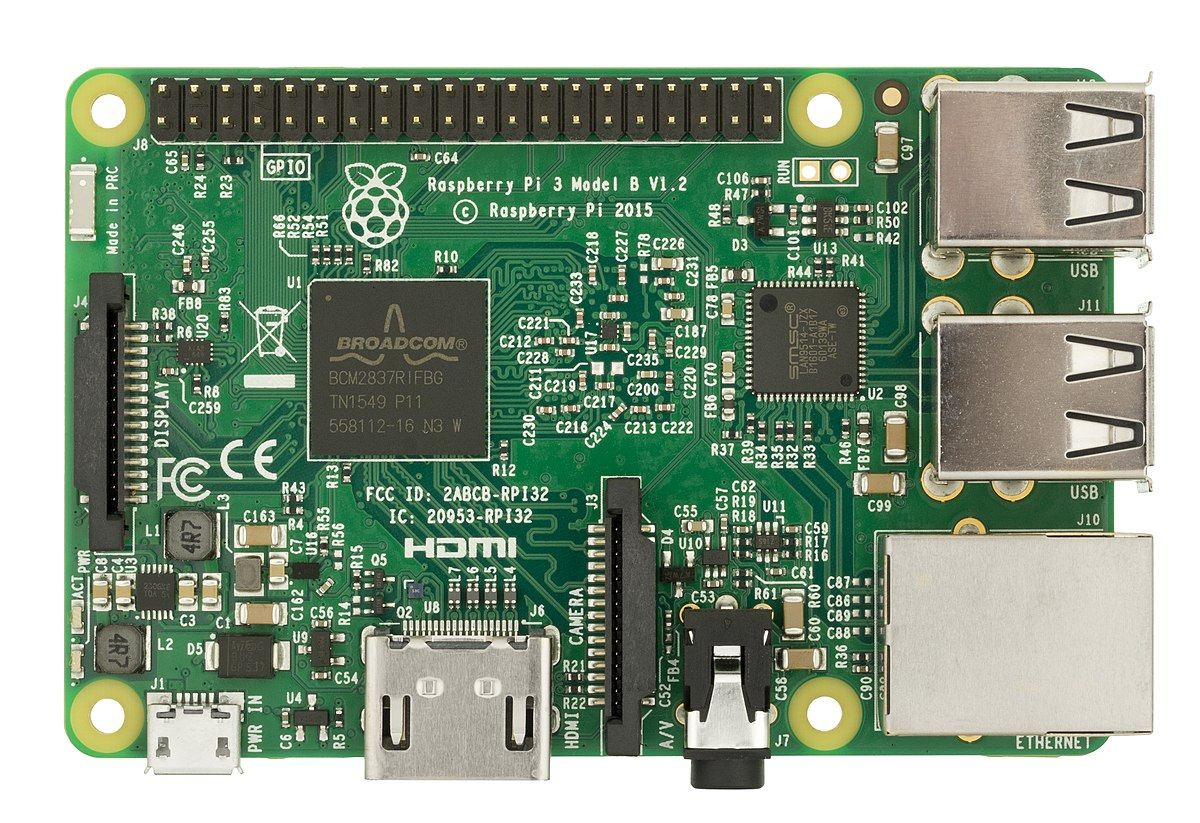
\includegraphics[width=0.7\textwidth]{images/rpi.jpg}
    \caption[Raspberry Pi 3]{Raspberry Pi 3 (obrázek převzat z~\url{https://en.wikipedia.org/wiki/Raspberry_Pi}).}
    \label{fig:rpi}
\end{figure}

Raspberry Pi je velmi rozšířený jednodeskový počítač. Jeho poslední verze, Raspberry Pi 3, je postavena na SoC Broadcom BCM2837 s~čtyřjádrovým procesorem ARM Cortex A53, který je až o~50 \% rychlejší než procesor předchozí verze \cite{rpi_benchoff}.

Dále nová verze přináší vlastní WiFi modul \cite{rpi_benchoff}, není tedy nutné se spoléhat na externí moduly. Kromě toho je možné počítač připojit k~síti pomocí Ethernetového portu. Ten je omezený na 100 Mb/s \cite{rpi_benchoff}, to by však vzhledem k~objemu dat přenášených mezi nadřazeným a podřízenými systémy nemělo představovat problém.

Deska také obsahuje čtyři USB a jeden HDMI port \cite{rpi_benchoff}. Ty nejsou pro implementovaný systém zásadní, nicméně při počáteční konfiguraci zařízení (například nastavení WiFi hesla) může být připojení monitoru a klávesnice pro některé uživatele pohodlnější než použití SSH či sériové linky. Připojený monitor se také hodí při řešení problémů se startem operačního systému.

Raspberry Pi 3 bohužel nemá vlastní bateriově zálohovaný RTC obvod a k~udržování času využívá protokol NTP \cite{rpi_rtc_ada}. K~tomu je však zapotřebí internetové připojení. Jelikož by zařízení mělo být možné používat i v~síti bez přístupu k~internetu, je nutné připojit externí RTC obvod, napřílad pomocí I2C sběrnice \cite{rpi_rtc_ada}. Poté je možné systémové hodiny synchronizovat bez internetového připojení pomocí tohoto obvodu.

S~počítačem je možné použít množství operačních systémů, z~nichž nejrozšířenější je pravděpodobně Raspbian, linuxový systém postavený na Debianu \cite{raspbian_faq}. Pro ten jsou dostupné všchny potřebné softwarové balíčky popsané v~sekci \ref{sec:an_plat}. Jelikož počítač nemá žádné vlastní úložiště, je nutné operační systém provozovat na vložené SD kartě \cite{rpi_benchoff}.

Jednou z~výhod tohoto počítače je obrovské množství podporovaných hardwarových periferií a knihoven pro ně. V~této práci pravděpodobně využiju pouze zmíněný RTC obvod, případné další rozšiřování systému (například o~vestavěný LCD displej) bude na Raspberry Pi pravděpodobně snadnější než na jiných platformách.

Kromě široké podpory je hlavní výhodou Raspberry Pi jeho cena. Poslední verze se pohybuje kolem 1200 Kč. K~celkovým nákladům na systém je ještě třeba připočítat cenu RTC obvodu a SD karty. Zde počítám s~použitím již připraveného modulu s~obvodem PCF8523 (pro bližší informace o~modulu viz \cite{rpi_rtc_ada}). Ten vyjde asi na 200 Kč. Jako úložiště by měla plně dostačovat 16GB SD karta, která se dá pořídit za 200 Kč. Celkové náklady na hardware systému se tedy měly pohybovat kolem 1600 Kč\footnote{Ceny převzaté z~obchodů Alza (\url{https://alza.cz}) a SnailShop(\url{www.snailshop.cz}), v~únoru 2018.}.

\subsection{Zybo Zynq-7000}
\label{sec:an_zyb}

\begin{figure}[h!]
    \centering
    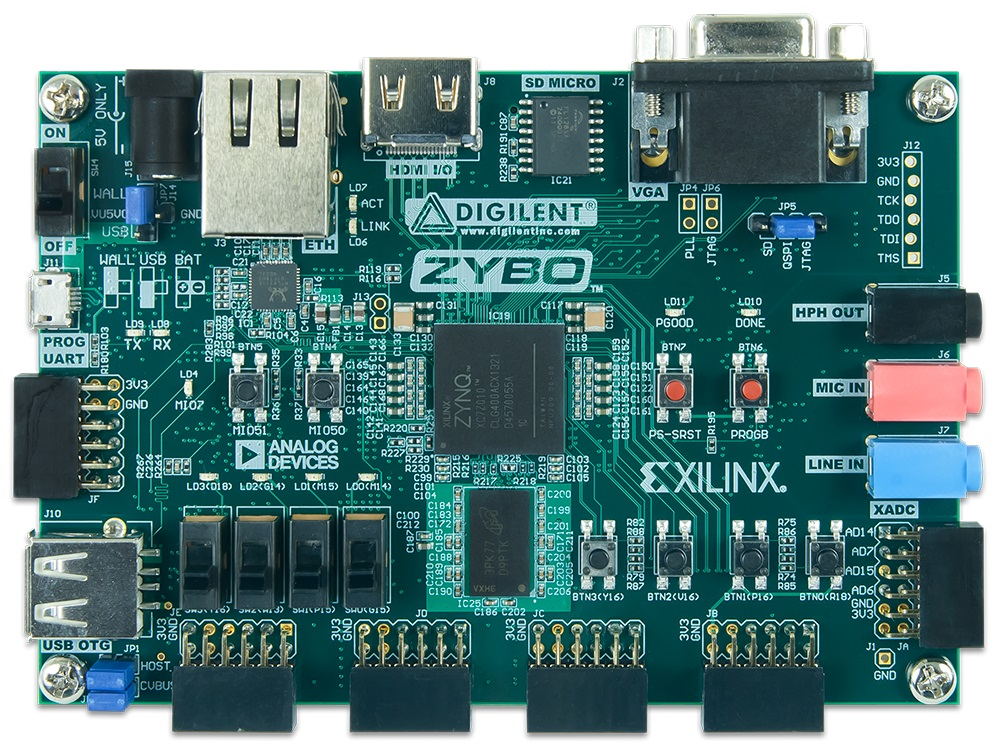
\includegraphics[width=0.7\textwidth]{images/zybo.jpg}
    \caption[Přípravek Zybo Zynq-7000]{Připravek Zybo Zynq-7000 (obrázek převzat z~\url{https://www.xilinx.com/products/boards-and-kits/1-4azfte.html}).}
    \label{fig:zybo}
\end{figure}

Tento přípravek od společnosti Digilent je postavený na SoC Xilinx Zynq Z-7010. Hlavní předností tohoto čipu je kombinace dvoujádrového procesoru ARM Cortex A9 s~FPGA odpovídající sérii Artix-7 \cite{zybo_man}. 

Díky tomu je možná těsná integraci mezi aplikací běžící na procesoru a výkonnými, úzce specializovanými moduly, které jsou syntetizované na FPGA. Tento přístup, kdy je hardware a software systému vyvíjen souběžně se označuje jako \textit{hardware/software codesign} \cite{hw_code}.

%dostupne operacni systemy -- petalinux, xilinux
Pro SoC ze série Zynq vznikla linuxová distribuce Xilinux, vycházející z~Ubuntu. Kromě plnohodnotného operačního systému (včetně například grafického rozhraní) poskytuje Xilinux také ovladače pro komunikaci s~FPGA pomocí AXI sběrnice \cite{xilibus}. K~tomu využívá \textcolor{magenta}{IP jádro Xilibus}, které funguje jako adaptér mezi \textcolor{green}{procesorem} a FPGA modulem (viz obrázek \ref{fig:xilibus}). Ten pak ke komunikaci může využívat standardni \textcolor{blue2}{FIFO} fronty a nemusí se zabývat AXI sběrnicí \cite{xilibus}.

\begin{figure}[h!]
    \centering
    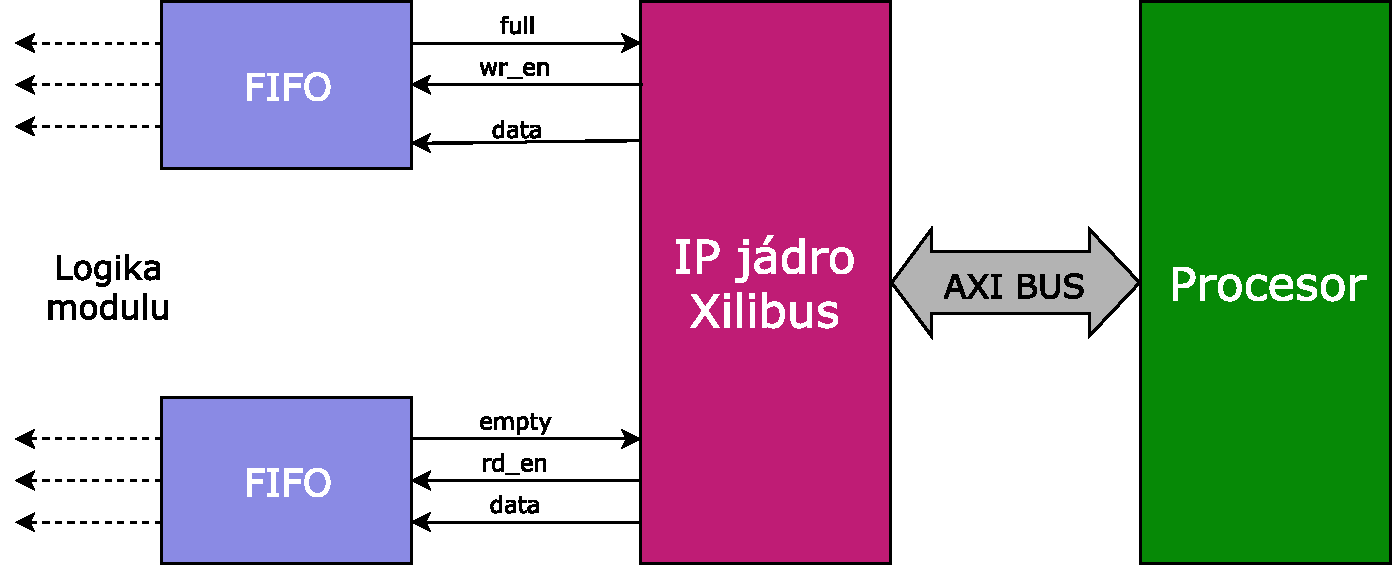
\includegraphics[width=\textwidth]{images/xilibus.pdf}
    \caption[Blokové schéma využití IP jádra Xilibus]{Blokové schéma využití IP jádra Xilibus \cite{xilibus}. Procesor přípravku komunikuje pomocí AXI sběrnice s~jádrem Xilibus. To požadovaná data zapíše či přečte z~FIFO fronty příslušného modulu.}
    \label{fig:xilibus}
\end{figure}

Jelikož Xilinux staví na Ubuntu (konkrétně na verzi 12.04 LTS \cite{xilibus}), neměl by být problém nainstalovat software potřebný pro provoz nadřazeného systému (viz sekci \ref{sec:an_plat}). 

Přípravek je možné připojiř k~síti pomocí Ethernetového portu, který podporuje rychlost až 1Gb/s \cite{zybo_man}. WiFi připojení by bylo možné realizovat pomocí USB modulu. Dále přípravek obsahuje HDMI a VGA port, audio konektory, čtyři tlačítka, čtyři přepínače a slot pro SD kartu \cite{zybo_man}.

Na přípravku je také k~dispozici 128 MB flash paměti \cite{zybo_man}, k~provozu tedy teoreticky není potřeba SD karta. Tato paměť by však pravděpodobně nestačila k~instalaci vhodného operačního systému a potřebného softwaru. I~zde by tedy bylo nutné použít SD kartu.

Stejně jako Raspberry Pi tato deska postrádá RTC obvod. Firma Digilent však dodává externí obvod, který lze připojit pomocí Pmod rozhraní \cite{pmod_rtc_man}. 

Nevýhodu této desky (především v~porovnání Raspberry Pi) je její cena. Ta se pohybuje okolo 4000 Kč\footnote{Cena podle produktové stránky \url{https://www.xilinx.com/products/boards-and-kits/1-4azfte.html}, v~únoru 2018.}. K~tomu je nutné přičíst náklady na SD kartu a RTC obvod, případně i WiFi modul. Cena celého zařízení by se tedy pohybovala v~rozmezí 4500 až 5000 Kč.

%bacha tady este na "As of 9/21/2017- the Zybo will be replaced by the Zybo Z7-10. We have created this guide to help you migrate your designs to the Zybo Z7. " ale nevim jestli to ma cenu resit ty desky se lisej minimalne (SoC je stejnej)
%^^linx: https://store.digilentinc.com/zybo-z7-zynq-7000-arm-fpga-soc-development-board/

\subsection{Závěr výberu platformy}

\begin{table}[h!]
\centering
\begin{tabular}{|c | c | c |} 
 \hline
 & \textbf{Raspberry Pi 3} & \textbf{Zybo Zynq-7000} \\
 \hline 
 SoC & Broadcom BCM2837 & Xilinx Zynq Z-7010 \\ 
 Procesor & ARM Cortex A53 & ARM Cortex A9 \\
 & 4 jádra, 1,2 GHz & 2 jádra, 650 MHz \\
 RAM & 1024 MB LPDDR2 & 512 MB DDR3 \\
 FPGA & -- & ekvivalent řady Artix-7 \\
 Úložiště & SD karta & 128 MB Flash, SD karta \\
 Síť & 100 Mb/s Ethernet, WiFi & až 1 Gb/s Ethernet \\
 Cena & 1200 Kč & 4000 Kč \\
 \hline
\end{tabular}
\caption[Srovnání platforem Raspberry Pi 3 a Zybo Zynq-7000]{Srovnání platforem Raspberry Pi 3 a Zybo Zynq-7000 \cite{rpi_benchoff, zybo_man}.}
\label{tab:plat_compare}
\end{table}

Jak vyplývá z~tabulky \ref{tab:plat_compare}, Raspberry Pi 3 poskytuje znatelně výkonnější procesor a více paměti za méně než třetinu ceny desky Zybo. Hlavní přidaná hodnota této platformy tedy spočívá v~integraci s~FPGA, ta má však v~případě této práce pouze velmi omezené využití. 

FPGA by bylo možné využít například k~šifrování úložiště, vzhledem k~předpokládáným objemům dat by však zrychlení oproti softwarovému šifrování neospravedlnilo vysokou cenu přípravku. Na druhou stranu vyšší výkon procesoru u~Raspberry Pi může mít pro nadřazený systém význam, například z~hlediska odezvy uživatelského rozhraní.

Jako platformu pro implementaci nadřazeného systému jsem tedy zvolil Raspberry Pi 3, především kvůli příznivé ceně, výrazně lepšímu poměru cena/výkon (pro tuto práci), a také kvůli podpoře a rozšiřitelnosti.

\subsection{Provoz aplikace na \textit{cloudové} platformě}
\label{sec:an_cloud}

V~této části bych chtěl popsat alternativu k~provozu systému na dedikovaném zařízení, a to možnost využít virtuální server na některé \textit{cloudové} platformě. Primární cíl práce je sice vytvořit nadřazený systém jako jednoúčelové zařízení (postavené na Raspberry Pi), nicméně provoz výsledné aplikace v~\textit{cloudu} může být v~určitých situacích vhodnější řešení.

Jedním z~možných uplatnění této varianty je monitorování více garážových komplexů. Místo lokálního nadřazeného systému by mohly všechny \textcolor{blue2}{podřízené systémy} z~každého komplexu komunikovat s~jedním \textcolor{magenta}{globálním systémem}, provozovaným na virtuálním serveru a dostupným z~internetu, jak je naznačeno na obrázku \ref{fig:aws}. Při tomto provozu je však nutnost mít registrovanou doménu a zabezpečit spojení podepsaným certifikátem.

Virtuální servery nabízí například firma DigitalOcean. Cena serveru závisí na počtu výpočetních jader, dostupně RAM a velikosti úložiště. Nejlevnější konfigurace přijde na 5 dolarů měsíčně a nabízí jednojádrový procesor, 1 GB RAM a 25 GB SSD \cite{digi_pricing}. Předpokládám, že tento výkon by stačil pro základní provoz systému, v~případě vyššího počtu podřízených systémů je však možnost zvyšovat dostupnou RAM a jádra CPU. 

S~těmito virtuálními servery lze použít řadu běžných linuxových operačních systémů jako Ubuntu, Debian či Fedora \cite{digi_droplets}, dostupnost softwaru potřebného pro spuštění aplikace tedy není problém.

Hlavní nevýhodou tohoto přístupu je poněkud složitější nasazení a spuštění systému. Registrace domény, získání certifikátu a základní konfigurace webového serveru se dá sice částečně automatizovat (viz zmiňovaný Certbot \cite{certbot}), pro většinu uživatelů bude však pravděpodobně snazší použít již připravené Raspberry Pi.

Také je složitější distribuovat adresu serveru s~nadřazeným systémem podřízeným systémům. V~místní síti může podřízený systém sám nalézt nadřazený systém testováním odpovědi zařízení v~síti na registrační požadavek. Pokud by však byl nadřazený systém dostupný pouze na internetové doméně, bylo by nutné ji ručně zadat každému podřízenému systému.

Další problém může představovat hlavní výhoda tohoto řešení, a to přístupnost serveru z~internetu. Ta významně zvyšuje \textit{attack surface} celého nadřazeného systému, zvlášt oproti alternativě využívající k~propojení systémů pouze Ethernet u~kterého má (na rozdíl od WiFi) provozovatel fyzický přehled o~připojených zařízeních.

\begin{figure}[h!]
    \centering
    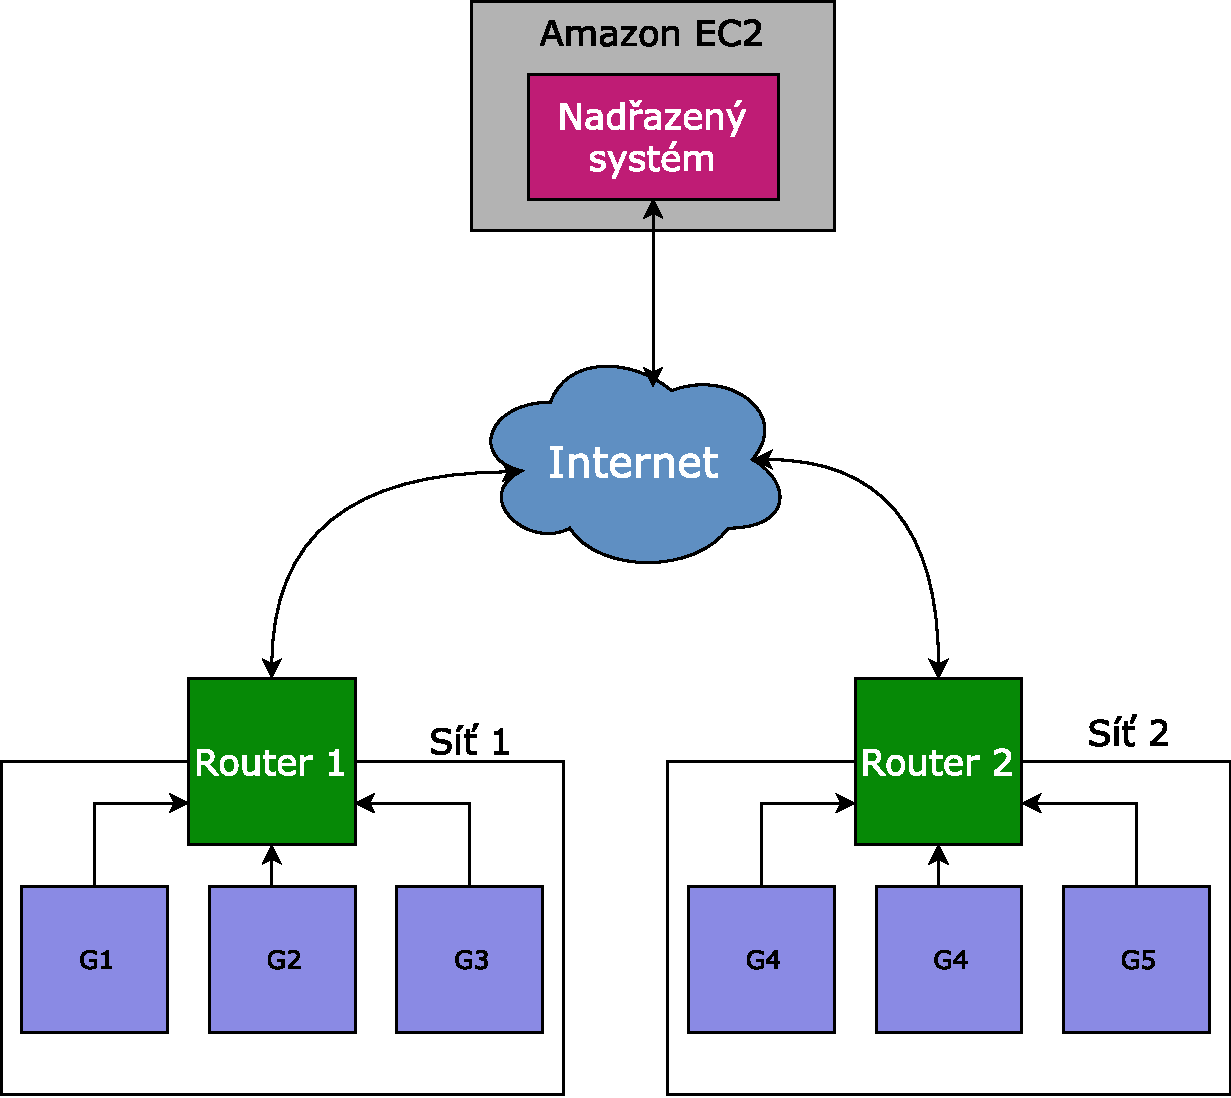
\includegraphics[width=\textwidth]{images/aws.pdf}
    \label{fig:aws}
    \caption[Struktura systému provozovaného na virtuálním serveru]{Struktura systému provozovaného na virtuálním serveru. Podřízené systémy nezasílají požadavky lokálnímu nadřazenému systému v~místní síti, ale globálnímu nadřazenému systému, který je veřejně přístupný na internetu.}
\end{figure}